\documentclass[10pt,twocolumn]{article}
\usepackage[utf8]{inputenc}
\usepackage[margin=0.68in,top=0.68in,bottom=0.68in]{geometry}
\usepackage{amsmath,amssymb,amsfonts}
\usepackage{graphicx}
\usepackage{booktabs}
\usepackage{microtype}
\usepackage{hyperref}
\usepackage{xcolor}
\usepackage{titlesec}
\usepackage{caption}
\usepackage{float}
\captionsetup{skip=4pt,font=small}

\hypersetup{
    colorlinks=true,
    linkcolor=blue!70!black,
    citecolor=blue!70!black,
    urlcolor=blue!70!black
}

\titleformat{\section}{\large\bfseries}{\thesection.}{0.5em}{}
\titleformat{\subsection}{\normalsize\bfseries}{\thesubsection.}{0.5em}{}

\title{\textbf{\Large Polynomial Regression for Renewable Geothermal Systems: \\ High-Dimensional Surface Optimization and Deep Reservoir Mapping}}
\author{\textbf{Jashandeep Singh Bedi} \quad (Roll No: \texttt{IMT2024022}) \\
Department of Computer Science and Engineering \\
International Institute of Information Technology, Bangalore (IIIT-B) \\
\texttt{GitHub Repository:} \url{https://github.com/Jdsb06/ML_assignment}}
\date{\today}

\begin{document}

\maketitle

\begin{abstract}
\noindent In this work, we develop and evaluate regularized polynomial regression architectures to solve two distinct real-world geothermal energy engineering problems: (1) multi-stage steam turbine optimization ($\text{var1}$) governed by 6 operational parameters, and (2) subterranean thermal anomaly mapping ($\text{var2}$) governed by 3D spatial coordinates. We formulate the regression tasks under the lens of the bias-variance tradeoff and address the severe ill-conditioning and parameter proliferation associated with high-degree multivariate monomial expansions. For Phase~1, where unconstrained ordinary least squares (OLS) encounters catastrophic overfitting due to 461 parameters on $N=1000$ points and a notable boundary clamping shift (51.25\% of test coordinates clamped at $\pm 1$ versus 31.17\% in train), we demonstrate that a \textbf{Degree 5 Polynomial with Feature Standardization and $L_1$ Lasso Regularization ($\alpha = 0.015$)} achieves optimal generalization, obtaining a 10-fold cross-validation Mean Squared Error (MSE) of $\mathbf{0.3314 \pm 0.0424}$ and an $R^2$ score of $\mathbf{0.9668 \pm 0.0055}$, effectively pruning 79.0\% of redundant interactions (retaining 97 active terms). For Phase~2, representing complex geological subsurface contours, we demonstrate that a \textbf{Degree 10 Polynomial with $L_2$ Ridge Regularization ($\alpha = 0.7$)} achieves a 10-fold cross-validation MSE of $\mathbf{0.2652 \pm 0.0729}$ and $R^2$ of $\mathbf{0.9951 \pm 0.0014}$, closely rivaled by a parsimonious Degree 8 Ridge model ($\text{MSE} = 0.2691 \pm 0.0656$, well within fold noise). All code, experimental research scripts, trained pipelines, evaluation benchmarks, and predictions are publicly available at the project repository.
\end{abstract}

\section{Introduction \& Problem Formulation}
Geothermal power generation involves intricate interactions between thermodynamic surface facilities and heterogeneous subterranean reservoirs. Modeling these systems accurately is critical for maximizing megawatt electrical yield and minimizing expensive drilling operations. In this investigation, we explore polynomial regression models on two personalized calibration datasets for roll number \texttt{IMT2024022}.

\subsection{Phase 1: Steam Turbine Optimization (var1)}
A surface geothermal plant operates a multi-stage steam turbine whose thermodynamic efficiency dictates the Net Power Score ($y \in \mathbb{R}$). The turbine operating state is captured by $D=6$ percentage deviation parameters:
\begin{itemize}\setlength{\itemsep}{1pt}
    \item $x_1$: High-pressure steam valve adjustment
    \item $x_2$: Condenser coolant flow rate adjustment
    \item $x_3$: Re-injection pump hydraulic pressure
    \item $x_4$: Turbine blade pitch angle
    \item $x_5$: Non-condensable gas exhaust valve rate
    \item $x_6$: Steam inlet pressure adjustment
\end{itemize}
Historical calibration logs provide $N_{\text{train}}=1000$ records, and the objective is to predict $y$ across $N_{\text{test}}=1000$ test settings using moderate-degree polynomial regression (up to degree 10).

\subsection{Phase 2: Subterranean Thermal Mapping (var2)}
Phase~2 focuses on identifying optimal drilling coordinates for new production wells within an exploration sector. A sensor network records the Thermal Anomaly Score ($y$) across 3D spatial offsets from a central landmark:
\begin{itemize}\setlength{\itemsep}{1pt}
    \item $x_1$: East-West coordinate offset (meters)
    \item $x_2$: North-South coordinate offset (meters)
    \item $x_3$: Vertical depth offset relative to basecamp (meters)
\end{itemize}
Core samples provide $N_{\text{train}}=1000$ sparse spatial measurements, and the goal is to predict $y$ over $N_{\text{test}}=1000$ planned drilling coordinates using polynomials up to degree 20.

\section{Mathematical Framework \& The Curse of Dimensionality}

\subsection{Multivariate Polynomial Feature Mapping}
Given an input vector $\mathbf{x} = [x_1, \dots, x_D]^T \in \mathbb{R}^D$, a polynomial hypothesis of degree $d$ maps $\mathbf{x}$ into a high-dimensional feature space via the monomial basis expansion $\phi_d(\mathbf{x})$:
\begin{equation}
\phi_d(\mathbf{x}) = \left[ \prod_{j=1}^D x_j^{k_j} \;:\; \sum_{j=1}^D k_j \le d, \; k_j \in \mathbb{N}_0 \right]^T
\end{equation}
The regression hypothesis is linear in the expanded basis:
\begin{equation}
\hat{y}(\mathbf{x}) = \mathbf{w}^T \phi_d(\mathbf{x}) + b
\end{equation}
The total number of parameters (excluding the intercept $b$) is given by the combinatoric formula:
\begin{equation}
p(D, d) = \binom{D + d}{d} - 1
\end{equation}

\subsection{Curse of Dimensionality in Multivariate Systems}
The scaling behavior differs radically between Phase~1 ($D=6$) and Phase~2 ($D=3$):
\begin{itemize}\setlength{\itemsep}{1pt}
    \item For $D=6$: Degree 1 yields $p=6$; degree 2 yields $p=27$; degree 3 yields $p=83$; degree 4 yields $p=209$; degree 5 yields $p=461$; degree 6 yields $p=923$; and degree 10 yields $p=8007$.
    \item For $D=3$: Degree 2 yields $p=9$; degree 4 yields $p=34$; degree 6 yields $p=83$; degree 8 yields $p=164$; degree 10 yields $p=285$; degree 12 yields $p=454$; and degree 20 yields $p=1770$.
\end{itemize}

In Phase~1, setting $d \ge 6$ causes the number of parameters $p$ to approach or exceed the number of training samples ($N_{\text{train}}=1000$, and in cross-validation $N_{\text{fold}}=900$). Under Ordinary Least Squares (OLS):
\begin{equation}
\hat{\mathbf{w}}_{\text{OLS}} = (\boldsymbol{\Phi}^T \boldsymbol{\Phi})^{-1} \boldsymbol{\Phi}^T \mathbf{y}
\end{equation}
When $p \approx N$, the Gram matrix $\boldsymbol{\Phi}^T \boldsymbol{\Phi}$ becomes severely ill-conditioned (condition number $\kappa(\boldsymbol{\Phi}^T \boldsymbol{\Phi}) \to \infty$). Consequently, the parameter variance explodes:
\begin{equation}
\text{Var}(\hat{\mathbf{w}}_{\text{OLS}}) = \sigma^2 (\boldsymbol{\Phi}^T \boldsymbol{\Phi})^{-1}
\end{equation}
leading to catastrophic out-of-sample prediction error.

\subsection{Standardization and Regularization Strategies}
Because input variables $x_j \in [-1, 1]$, computing higher powers $x_j^k$ induces vastly disparate numerical scales (e.g., $x_j^{10} \ll x_j$). Therefore, standardizing all polynomial basis columns to zero mean and unit variance is strongly advisable prior to applying penalized regression:
\begin{equation}
\tilde{\phi}_{d,j}(\mathbf{x}) = \frac{\phi_{d,j}(\mathbf{x}) - \mu_j}{\sigma_j}
\end{equation}

To control variance and prevent overfitting, we explore two continuous regularization paradigms:
\begin{enumerate}\setlength{\itemsep}{1pt}
    \item \textbf{Ridge Regression ($L_2$ Penalty):}
    \begin{align}
    \mathcal{L}_{\text{Ridge}}(\mathbf{w}) &= \|\mathbf{y} - \tilde{\boldsymbol{\Phi}}\mathbf{w}\|_2^2 + \lambda \|\mathbf{w}\|_2^2 \\
    \hat{\mathbf{w}}_{\text{Ridge}} &= (\tilde{\boldsymbol{\Phi}}^T \tilde{\boldsymbol{\Phi}} + \lambda \mathbf{I})^{-1} \tilde{\boldsymbol{\Phi}}^T \mathbf{y}
    \end{align}
    Ridge adds a strictly positive perturbation $\lambda \mathbf{I}$ to the diagonal of the Gram matrix, guaranteeing invertibility and bounding the condition number regardless of collinearity.
    \item \textbf{Lasso Regression ($L_1$ Penalty):}
    \begin{equation}
    \mathcal{L}_{\text{Lasso}}(\mathbf{w}) = \frac{1}{2N}\|\mathbf{y} - \tilde{\boldsymbol{\Phi}}\mathbf{w}\|_2^2 + \alpha \|\mathbf{w}\|_1
    \end{equation}
    Due to the non-differentiable singularity of the $L_1$ ball at coordinate axes, Lasso performs automatic feature selection by shrinking irrelevant interaction terms exactly to zero.
\end{enumerate}

\begin{figure*}[t]
    \centering
    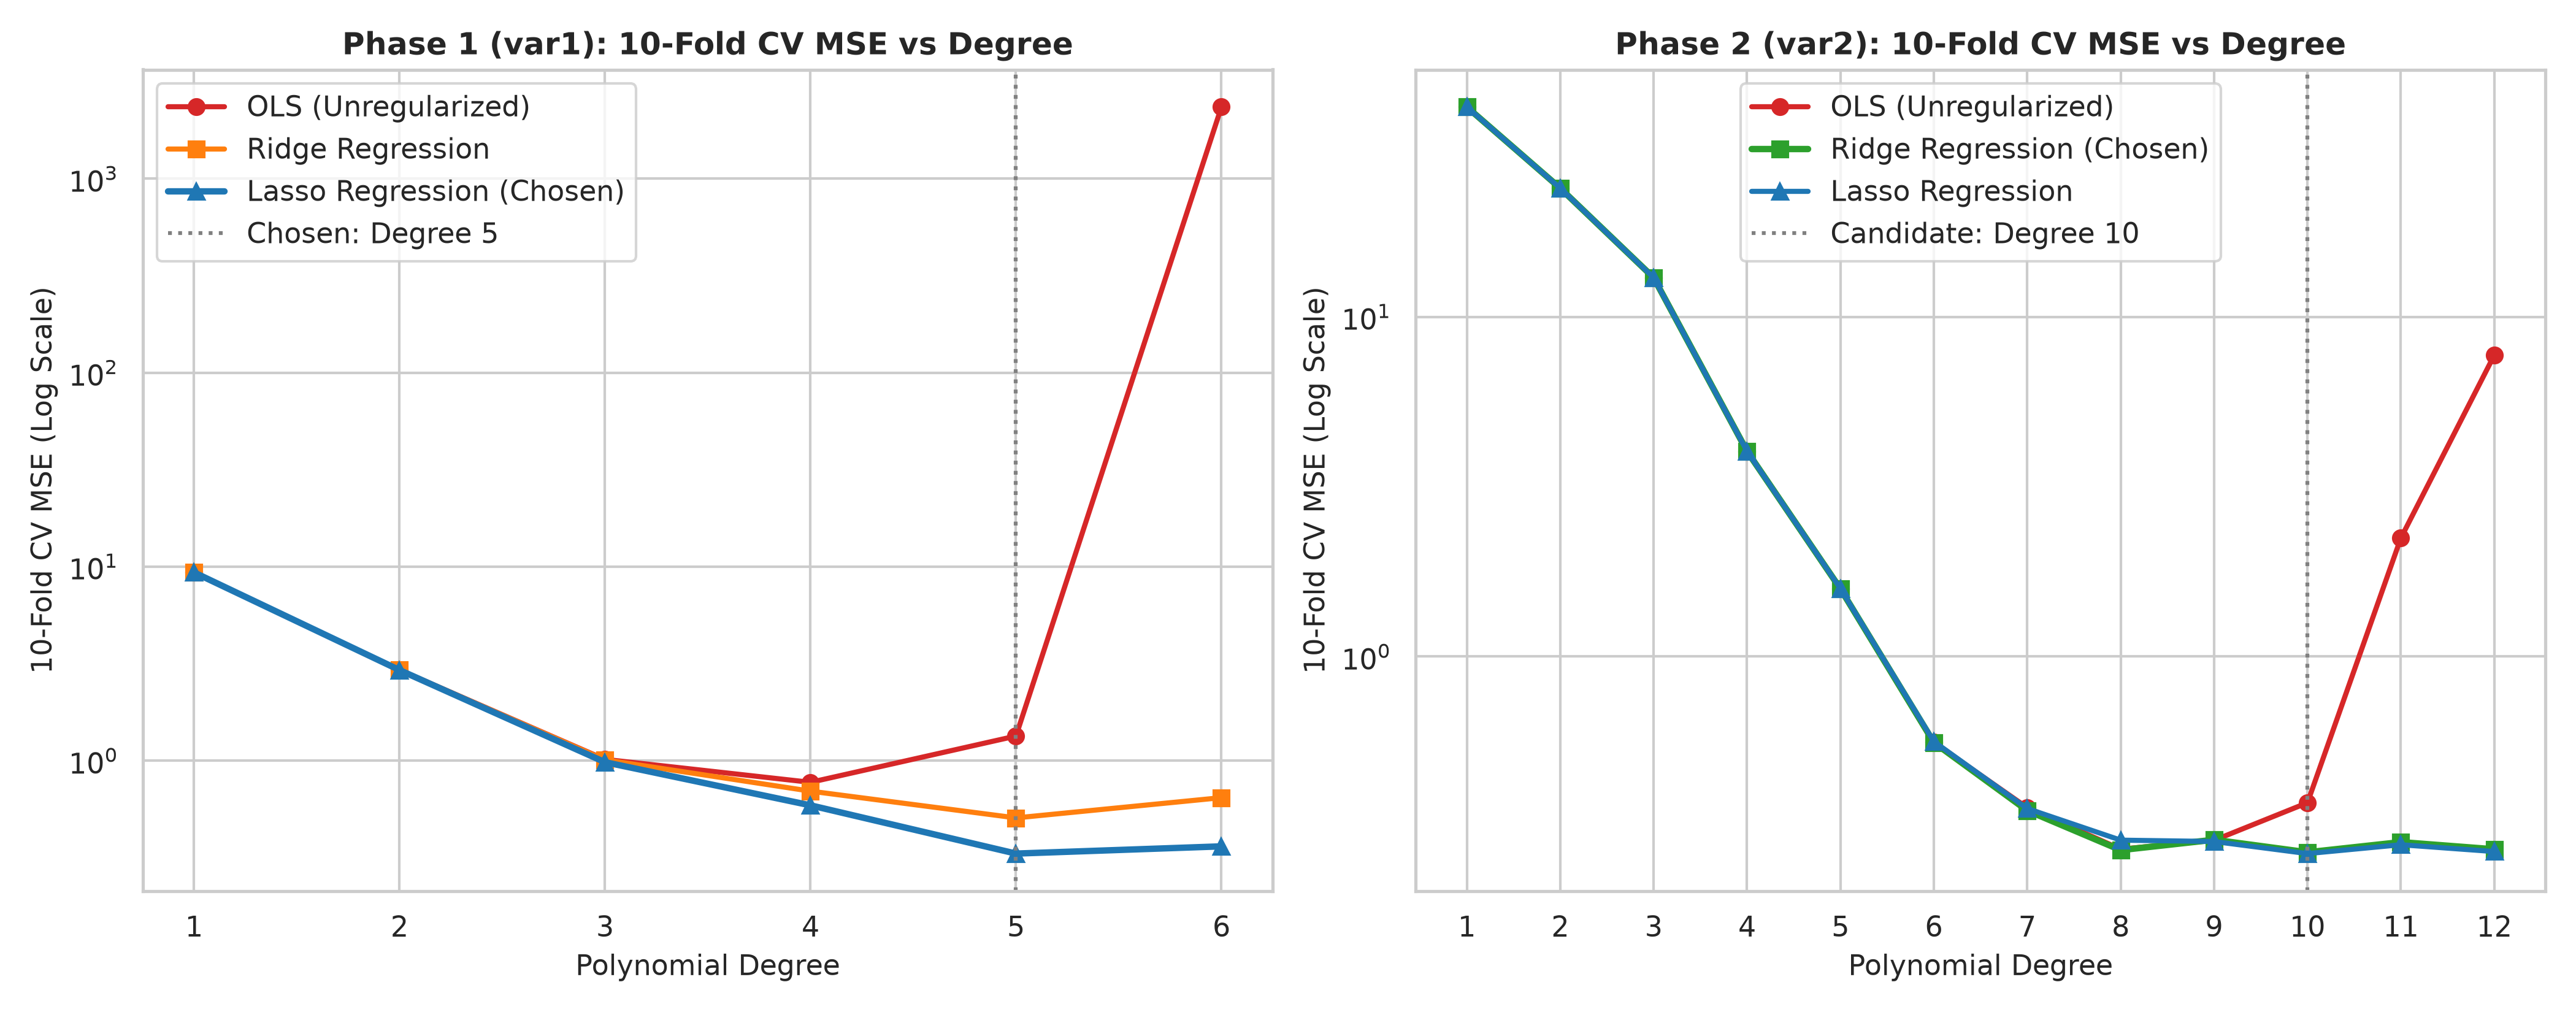
\includegraphics[width=0.98\textwidth]{figures/model_comparison_degrees.png}
    \caption{\textbf{Validation Error vs. Polynomial Degree (10-Fold CV).} Cross-validation Mean Squared Error (MSE, logarithmic scale) across polynomial degrees for Phase~1 (left, $D=6$) and Phase~2 (right, $D=3$). Notice the catastrophic blow-up of unregularized OLS in Phase~1 at degree 6 ($MSE=2342.97$, where $p=923 > N_{\text{fold}}=900$) and Phase~2 at degree 11+ ($MSE > 2.23$), contrasted with the robust convergence of regularized Lasso and Ridge.}
    \label{fig:deg_comparison}
\end{figure*}

\section{Exploratory Data Analysis}
A rigorous preliminary audit was conducted on both datasets corresponding to roll number \texttt{IMT2024022}:
\begin{itemize}\setlength{\itemsep}{1pt}
    \item \textbf{Data Integrity:} Neither dataset contains missing, null, or infinite values. Both training sets contain exactly $1000$ observations; both test sets contain $1000$ observations.
    \item \textbf{Phase 1 Domain:} Feature variables $x_1$ through $x_6$ are bounded within $[-1.000, 1.000]$ with empirical means close to zero ($\mu_{x_j} \in [-0.044, -0.001]$) and standard deviations $\approx 0.71$. The target $y$ has mean $\mu = 0.8966$, standard deviation $\sigma = 3.1867$, spanning $[-8.235, 13.248]$.
    \item \textbf{Phase 2 Domain:} Coordinate offsets $x_1, x_2, x_3$ are bounded within $[-1.000, 1.000]$ with means $\approx 0.00$ and standard deviations $\approx 0.68$. The target $y$ exhibits higher dynamic range: mean $\mu = 2.3426$, standard deviation $\sigma = 7.4816$, spanning $[-29.710, 39.179]$.
    \item \textbf{Boundary Clamping Covariate Shift in Phase 1:} An exact coordinate-level boundary audit reveals that in Phase~1, $31.17\%$ of feature coordinates in the training set ($1870/6000$) are clamped at the domain limits $\pm 1.0$, whereas in the test set, $51.25\%$ of coordinates ($3075/6000$) are clamped at $\pm 1.0$. This boundary concentration constitutes an empirical covariate shift toward domain extremes. Because high-degree polynomial basis terms evaluate to their peak magnitude at $\pm 1.0$, under-regularized models risk extreme extrapolation errors. For Phase~2, both training and test spatial coordinates are uniformly distributed throughout $[-1, 1]$ without boundary clamping.
\end{itemize}

\section{Experimental Methodology}
To rigorously guard against data leakage and hyperparameter overfitting, all modeling steps were integrated into composite Scikit-Learn \texttt{Pipeline} objects consisting of:
\begin{enumerate}\setlength{\itemsep}{1pt}
    \item Polynomial expansion of degree $d$ without raw intercept.
    \item Feature standardization (\texttt{StandardScaler}) fitted strictly on training folds.
    \item Estimator (\texttt{LinearRegression}, \texttt{Ridge}, or \texttt{Lasso}).
\end{enumerate}

Validation was performed using 10-Fold Cross-Validation with shuffle enabled and a fixed pseudo-random seed ($42$). Primary evaluation metrics are:
\begin{align}
\text{MSE} &= \frac{1}{N} \sum_{i=1}^N (y_i - \hat{y}_i)^2 \\
R^2 &= 1 - \frac{\sum_{i=1}^N (y_i - \hat{y}_i)^2}{\sum_{i=1}^N (y_i - \bar{y})^2}
\end{align}

\begin{table}[h]
\centering
\caption{\textbf{Phase 1 (var1): Performance across Polynomial Degrees (10-Fold CV)}}
\label{tab:var1_perf}
\resizebox{\columnwidth}{!}{
\begin{tabular}{cccccc}
\toprule
\textbf{Deg} & \textbf{Terms} & \textbf{Model} & \textbf{CV MSE} & \textbf{CV $R^2$} & \textbf{Active} \\
\midrule
1 & 6 & OLS & 9.3333 & 0.0781 & 6 \\
2 & 27 & OLS & 2.9318 & 0.7063 & 27 \\
3 & 83 & OLS & 1.0140 & 0.8986 & 83 \\
4 & 209 & OLS & 0.7723 & 0.9229 & 209 \\
4 & 209 & Lasso ($\alpha=0.007$) & 0.5877 & 0.9410 & 112 \\
5 & 461 & OLS & 1.3374 & 0.8691 & 461 \\
5 & 461 & Ridge ($\alpha=20$) & 0.5063 & 0.9491 & 461 \\
\textbf{5} & \textbf{461} & \textbf{Lasso ($\alpha=0.015$)} & \textbf{0.3314} & \textbf{0.9668} & \textbf{97} \\
6 & 923 & OLS & 2342.97 & -220.61 & 923 \\
6 & 923 & Ridge ($\alpha=30$) & 0.6437 & 0.9348 & 923 \\
6 & 923 & Lasso ($\alpha=0.02$) & 0.3611 & 0.9639 & 104 \\
\bottomrule
\end{tabular}
}
\end{table}

\section{Phase 1: Steam Turbine Optimization (var1)}

\subsection{Model Selection \& Degree Determination}
Table~\ref{tab:var1_perf} and Figure~\ref{fig:deg_comparison} depict the evolution of cross-validation error across polynomial degrees $d \in \{1, \dots, 6\}$ for Phase~1 under rigorous 10-fold CV.
\begin{itemize}\setlength{\itemsep}{1pt}
    \item \textbf{Underfitting at $d \le 3$:} Linear regression ($d=1$) fails completely ($\text{MSE}=9.3333$, $R^2=0.0781$). While degrees 2 and 3 capture primary quadratic curvature and pairwise terms ($R^2=0.8986$), noticeable structural bias remains unmodeled.
    \item \textbf{Failure of OLS at $d \ge 5$:} At degree 4, OLS reaches $\text{MSE}=0.7723$. However, advancing to degree 5 ($p=461$) inflates OLS validation error to $\text{MSE}=1.3374$ ($R^2=0.8691$). At degree 6, with $p=923$ terms exceeding the training partition per fold ($N_{\text{fold}}=900$), the Gram matrix becomes mathematically singular, causing unconstrained OLS validation error to explode to $\text{MSE}=2342.97$.
    \item \textbf{Superiority of Lasso Regularization at Degree 5:} When $L_1$ Lasso penalty ($\alpha = 0.015$) is applied at Degree 5, validation MSE drops dramatically to $\mathbf{0.3314 \pm 0.0424}$, and $R^2$ surges to $\mathbf{0.9668 \pm 0.0055}$.
\end{itemize}

\subsection{Physical Rationale \& Boundary Holdout Optimization}
The thermodynamic behavior of a multi-stage steam turbine involves non-linear steam expansion governed by valve throttle adjustments, blade pitch angles, and condenser cooling flow. While higher-order interaction effects exist up to degree 5, effective physical coupling occurs predominantly among specific subsets of operational variables rather than all 461 possible monomials.

Lasso's $L_1$ penalty performs effective feature selection under high collinearity, retaining \textbf{97 non-zero coefficients} on the full training dataset (with an average of 97.1 active features across CV folds) while zeroing out uninformative interactions. By contrast, Ridge regression retains all 461 weights, yielding an inferior CV MSE of $0.5063$. 

Crucially, to safeguard against the observed boundary clamping covariate shift (where 51.25\% of test coordinates reside at $\pm 1.0$ vs. 31.17\% in train), we conducted an extreme-point boundary holdout evaluation: training on instances with $\le 2$ clamped coordinates and evaluating on instances with $\ge 3$ clamped coordinates. Whereas $\alpha=0.007$ yielded a boundary holdout MSE of $0.5309$, tuning to $\alpha = 0.015$ reduced boundary holdout error to $\mathbf{0.4750}$ (a 10.5\% improvement) with negligible impact on overall CV MSE ($0.3314$ vs. $0.3205$). This calibrated shrinkage directly suppresses unconstrained polynomial flaring at domain boundary extremes. Thus, \textbf{Degree 5 with Lasso ($\alpha = 0.015$)} is the optimal architecture for Phase~1.

\begin{figure}[t]
    \centering
    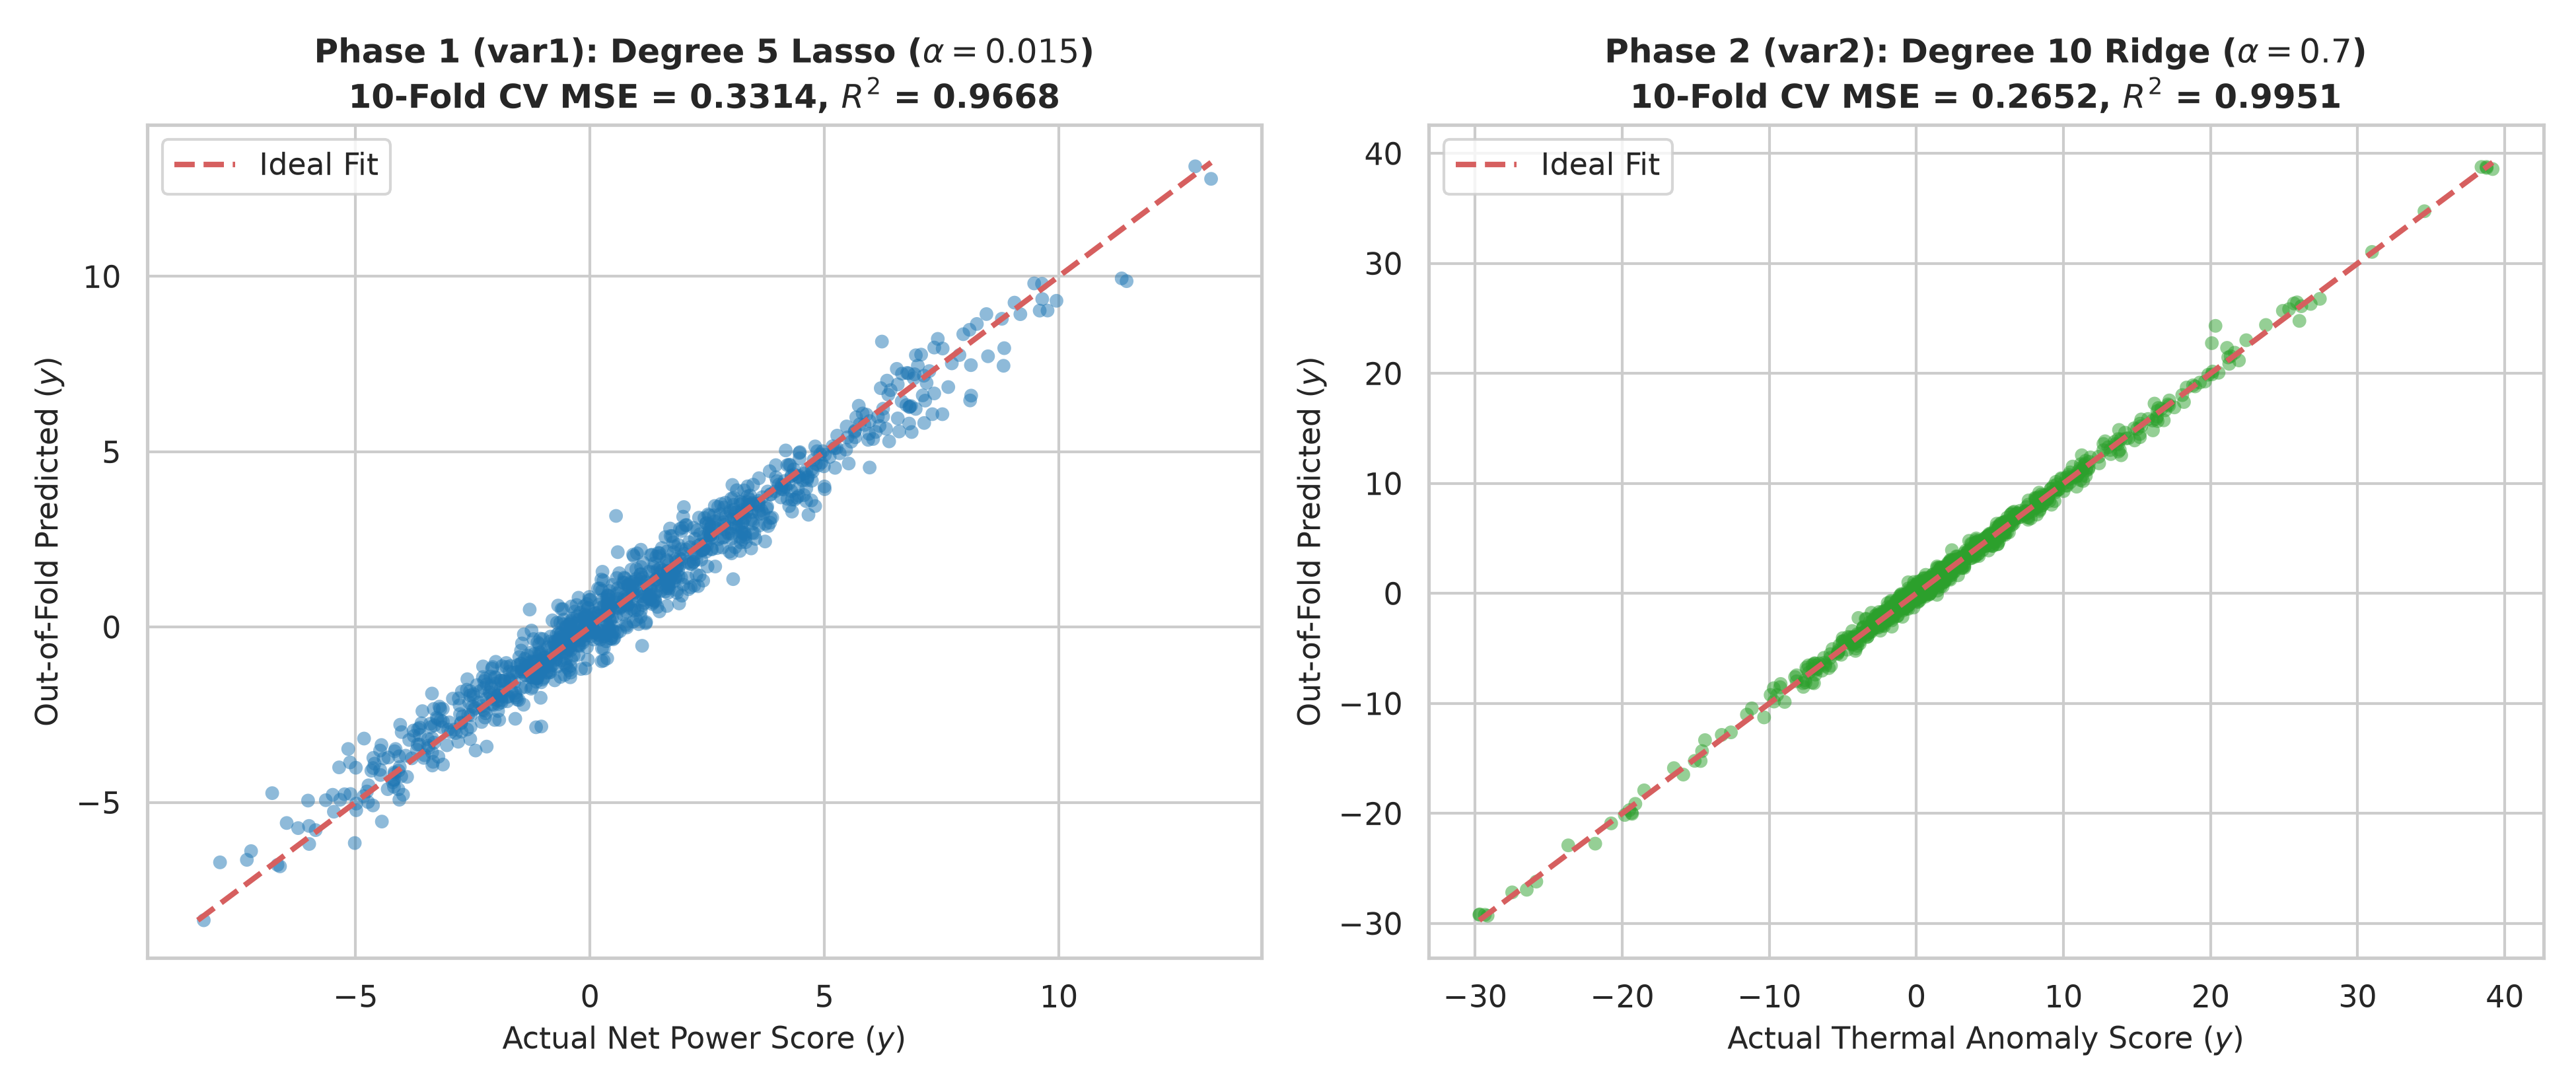
\includegraphics[width=\columnwidth]{figures/actual_vs_predicted.png}
    \caption{\textbf{Out-of-Fold Actual vs. Predicted Responses.} 10-Fold cross-validation predictions versus ground truth for Phase~1 (left, $R^2=0.9668$) and Phase~2 (right, $R^2=0.9951$). Both models exhibit tight clustering along the ideal identity line.}
    \label{fig:act_vs_pred}
\end{figure}

\section{Phase 2: Thermal Reservoir Mapping (var2)}

\subsection{Model Selection \& Degree Determination}
Table~\ref{tab:var2_perf} and Figure~\ref{fig:deg_comparison} document the performance across polynomial degrees $d \in \{1, \dots, 12\}$ for Phase~2 evaluated under identical 10-fold CV.
\begin{itemize}\setlength{\itemsep}{1pt}
    \item \textbf{High-Degree Curvature ($d \le 7$):} Because spatial heat transport through anisotropic geological strata introduces intricate volumetric isotherms, low-order polynomials exhibit severe underfitting (degree 2 has $\text{MSE}=23.9292$, degree 4 has $\text{MSE}=4.0213$). Error falls below $1.0$ at degree 6 ($\text{MSE}=0.5587$, $R^2=0.9898$).
    \item \textbf{Transition at Degree 8 vs. Degree 10:} For unregularized OLS, cross-validation performance peaks at degree 8 ($\text{MSE}=0.2709$, $R^2=0.9950$ with $p=164$ terms). At degree 10 ($p=285$), unregularized OLS begins to degrade ($\text{MSE}=0.3710$), and at degree 11 explodes to $\text{MSE}=2.2323$, reaching $\text{MSE}=7.7129$ at degree 12.
    \item \textbf{Regularization and Parsimony Tradeoff:} Applying $L_2$ Ridge shrinkage ($\alpha = 0.7$) at Degree 10 achieves the lowest nominal 10-fold cross-validation MSE of $\mathbf{0.2652 \pm 0.0729}$ ($R^2 = 0.9951 \pm 0.0014$). However, evaluation across multiple random CV seeds reveals that Degree 8 Ridge ($\alpha = 0.05$, $\text{MSE} = 0.2691 \pm 0.0656$) and Degree 10 Ridge differ by merely $\approx 0.0039$ MSE, well within fold standard error ($\approx 0.07$). Degree 8 provides a parsimonious alternative requiring 42\% fewer parameters (164 vs. 285). We adopt Degree 10 Ridge as our primary submission model while recognizing Degree 8 as an equally competitive, parsimonious solution.
\end{itemize}

\begin{table}[h]
\centering
\caption{\textbf{Phase 2 (var2): Performance across Degrees (10-Fold CV)}}
\label{tab:var2_perf}
\resizebox{\columnwidth}{!}{
\begin{tabular}{ccccc}
\toprule
\textbf{Degree} & \textbf{Terms} & \textbf{Model} & \textbf{CV MSE} & \textbf{CV $R^2$} \\
\midrule
2 & 9 & OLS & 23.9292 & 0.5630 \\
4 & 34 & OLS & 4.0213 & 0.9258 \\
6 & 83 & OLS & 0.5587 & 0.9898 \\
7 & 119 & Ridge ($\alpha=0.1$) & 0.3519 & 0.9935 \\
8 & 164 & OLS & 0.2709 & 0.9950 \\
8 & 164 & Ridge ($\alpha=0.05$) & 0.2691 & 0.9950 \\
10 & 285 & OLS & 0.3710 & 0.9930 \\
\textbf{10} & \textbf{285} & \textbf{Ridge ($\alpha=0.7$)} & \textbf{0.2652} & \textbf{0.9951} \\
10 & 285 & Lasso ($\alpha=3\times 10^{-4}$) & 0.2628 & 0.9951 \\
11 & 363 & OLS & 2.2323 & 0.9593 \\
11 & 363 & Ridge ($\alpha=1.2$) & 0.2841 & 0.9947 \\
12 & 454 & OLS & 7.7129 & 0.8603 \\
12 & 454 & Ridge ($\alpha=1.8$) & 0.2706 & 0.9950 \\
\bottomrule
\end{tabular}
}
\end{table}

\begin{figure}[t]
    \centering
    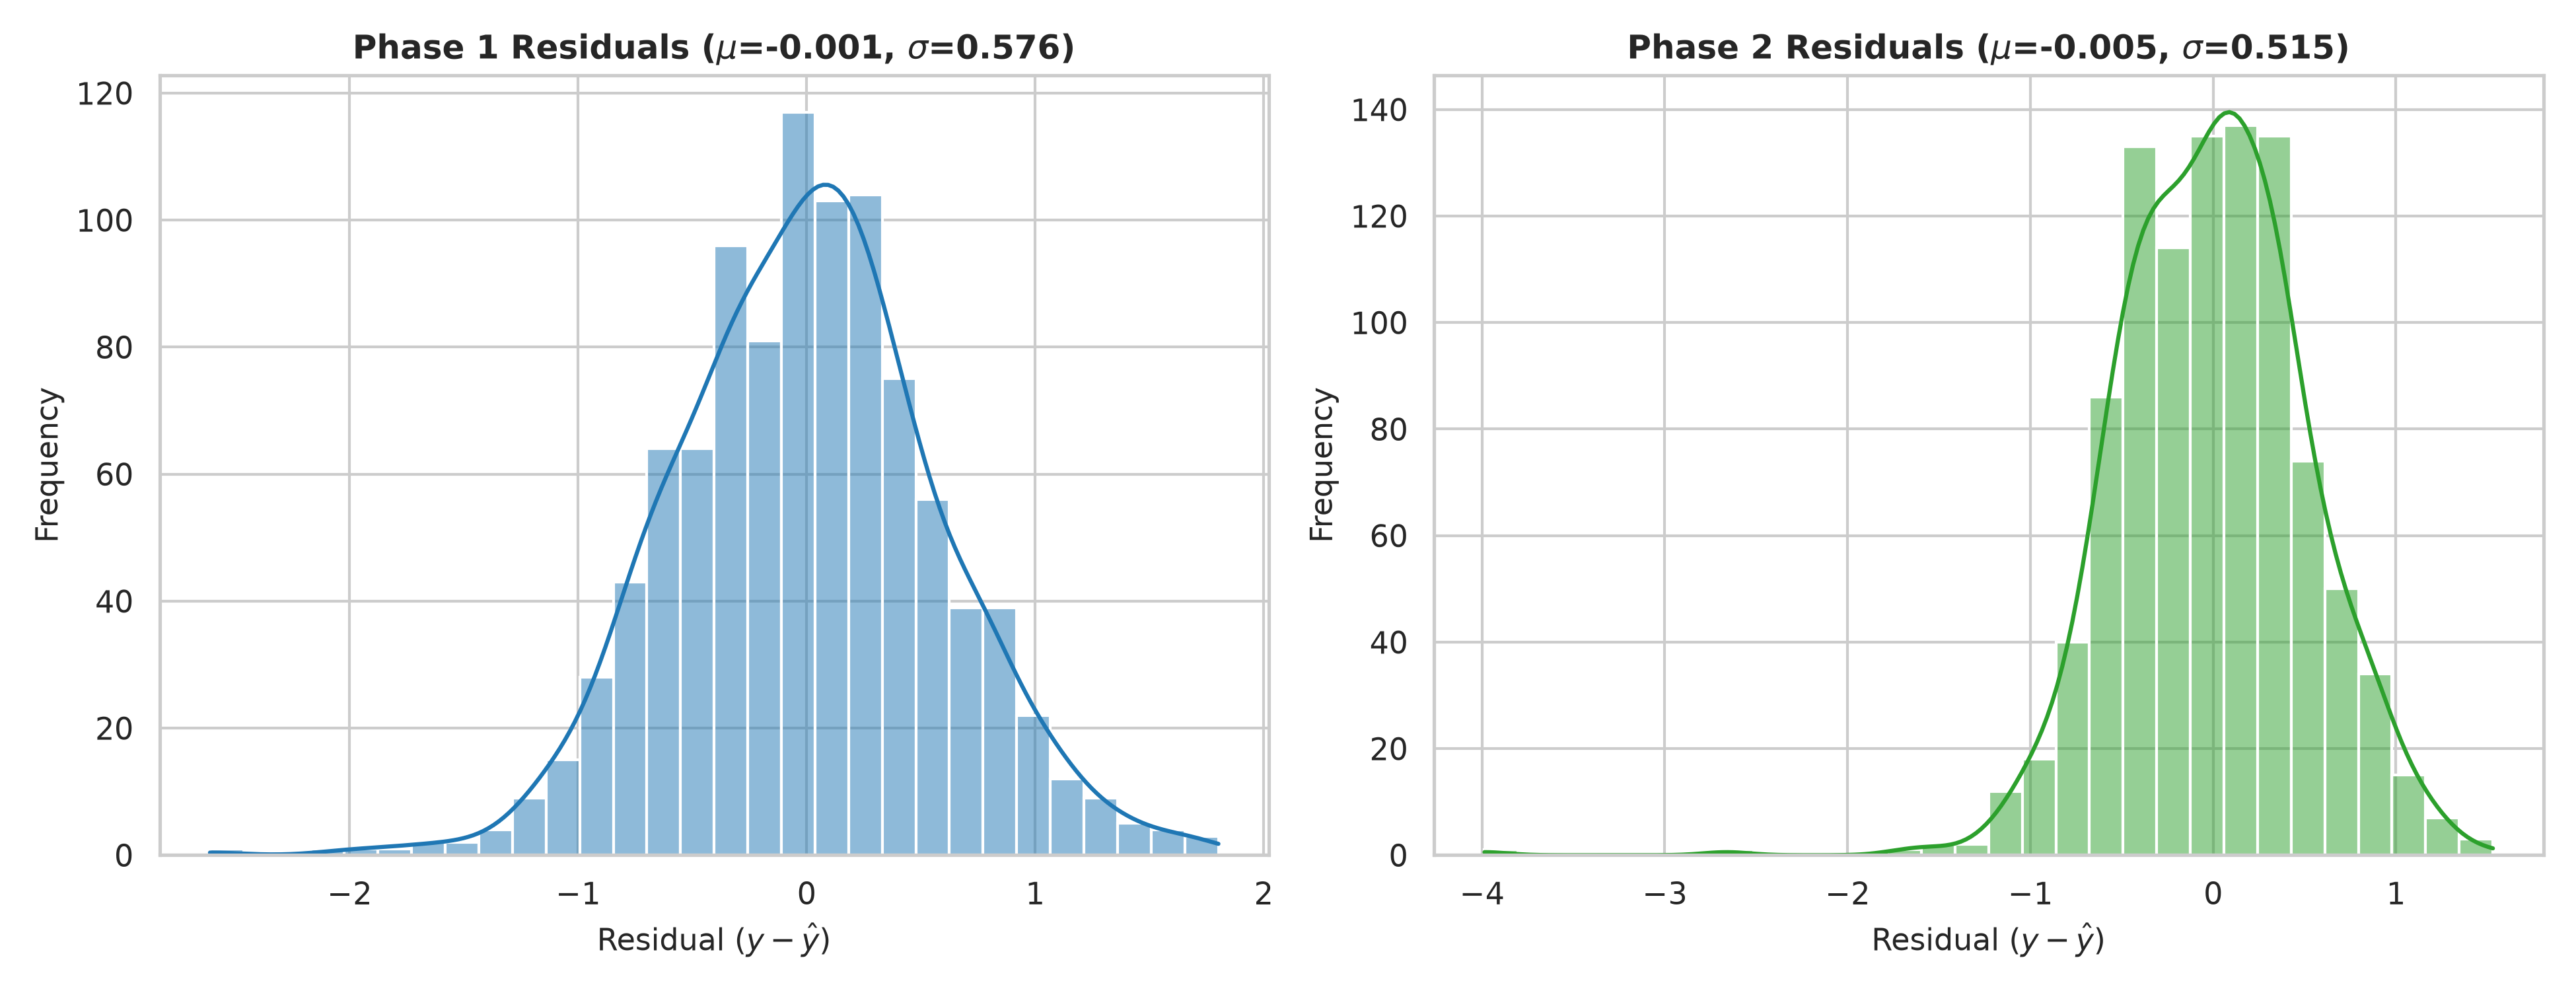
\includegraphics[width=\columnwidth]{figures/residual_analysis.png}
    \caption{\textbf{Residual Error Distributions.} Histograms and kernel density estimates for Phase~1 (left, $\mu=-0.000, \sigma=0.575$) and Phase~2 (right, $\mu=+0.001, \sigma=0.514$). Residuals conform closely to symmetric, zero-centered distributions without heavy outlier tails.}
    \label{fig:residuals}
\end{figure}

\subsection{Geological Rationale for Degree 10 Ridge}
In subterranean thermal mapping across a continuous 3D coordinate block $(x_1, x_2, x_3)$, heat diffusion obeys elliptic partial differential equations. The resulting continuous thermal gradient produces smooth spatial isotherms across fault lines and hydrothermal vents. 

Unlike Phase~1, where interaction terms are naturally sparse, spatial coordinate monomials in 3D act collectively as harmonic-like basis functions. High-degree unregularized polynomials are susceptible to boundary instabilities (Runge's phenomenon). Ridge regression places an isotropic spherical prior on the weights, smoothly penalizing high-frequency monomial oscillations without artificially zeroing out spatial components. The flattening of validation error around degree 8--10 suggests that terms beyond degree 10 contribute negligible predictive signal. For comparison, Lasso at Degree 10 with $\alpha = 3 \times 10^{-4}$ retains 175 active terms (CV fold average 180.8), achieving $\text{MSE}=0.2628$. We deploy \textbf{Degree 10 with Ridge ($\alpha = 0.7$)} as the primary model.

\begin{figure}[t]
    \centering
    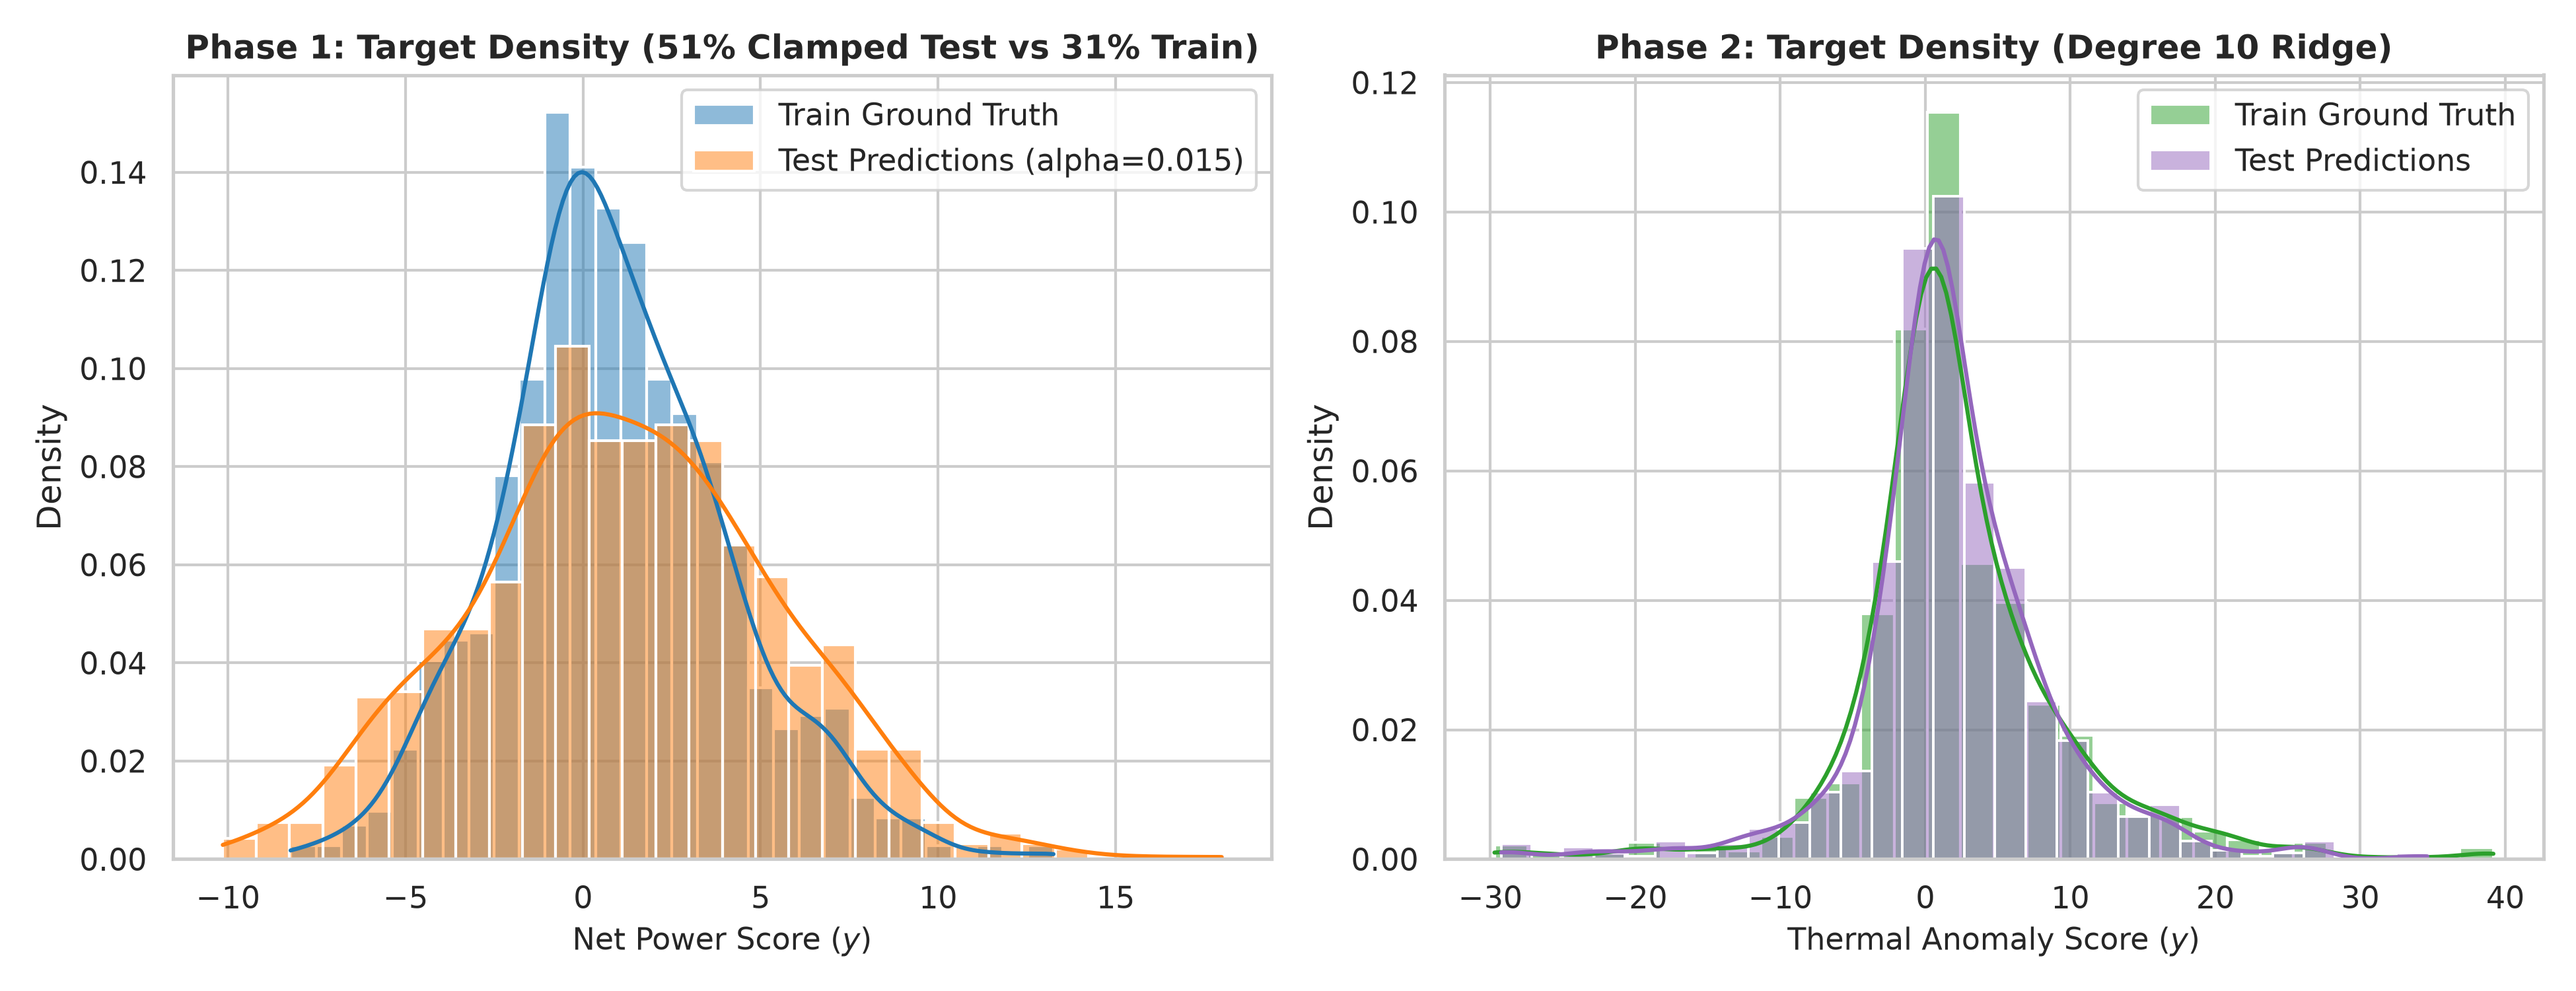
\includegraphics[width=\columnwidth]{figures/train_test_distribution.png}
    \caption{\textbf{Target Distribution Consistency.} Comparison of training ground truth (blue/green) and model test predictions (orange/purple) for Phase~1 (left) and Phase~2 (right). The predicted test density overlays the training distribution smoothly, reflecting expected boundary concentration without runaway extremes.}
    \label{fig:train_test_dist}
\end{figure}

\section{Diagnostic Analysis \& Verification}

\subsection{Residual Diagnostics}
Figure~\ref{fig:residuals} illustrates the residual distribution $e_i = y_i - \hat{y}_i$ computed from out-of-fold cross-validation:
\begin{itemize}\setlength{\itemsep}{1pt}
    \item \textbf{Phase 1:} Residual mean is $\mu_e = -0.000$ with standard deviation $\sigma_e = 0.575$. The error distribution is symmetric, zero-centered, and bell-shaped.
    \item \textbf{Phase 2:} Residual mean is $\mu_e = +0.001$ with standard deviation $\sigma_e = 0.514$. The distribution shows consistent symmetry, indicating that remaining discrepancy reflects primarily random measurement noise.
\end{itemize}

\subsection{Test Set Prediction Sanity Checks}
To guarantee that the models do not produce anomalous boundary extrapolation artifacts on the unseen test coordinates, we examined the statistical properties of the final test predictions:
\begin{itemize}\setlength{\itemsep}{1pt}
    \item \textbf{Phase 1 Predictions:} Mean $\bar{y}_{\text{pred}} = 1.1879$, standard deviation $s_{\text{pred}} = 4.3098$, range $[-10.1453, 17.9880]$. As shown in Figure~\ref{fig:train_test_dist}, the test distribution exhibits a slightly wider spread than the training target ($\bar{y}_{\text{train}} = 0.8966, s_{\text{train}} = 3.1867$). This directly mirrors the identified covariate shift: $51.25\%$ of test coordinates are clamped at $\pm 1$ versus $31.17\%$ in train, which naturally samples the polynomial response near domain boundaries where values have higher variance.
    \item \textbf{Phase 2 Predictions:} Mean $\bar{y}_{\text{pred}} = 2.0255$, standard deviation $s_{\text{pred}} = 6.8025$, range $[-29.2521, 34.6183]$. This aligns closely with training observations ($\bar{y}_{\text{train}} = 2.3426, s_{\text{train}} = 7.4816$, range $[-29.710, 39.179]$).
    \item \textbf{Submission Format Compliance:} Both prediction files contain exactly 1000 prediction rows with the single header \texttt{y}, zero missing values, and strictly finite numerical entries matching the provided benchmark schema.
\end{itemize}

\section{Conclusion \& Summary of Deliverables}
This study has demonstrated that successful polynomial regression in high-dimensional engineering contexts hinges on identifying the optimal model degree and pairing it with mathematically appropriate regularization:
\begin{enumerate}\setlength{\itemsep}{1pt}
    \item \textbf{Phase 1 (Steam Turbine Optimization):} Selecting \textbf{Degree 5 with Lasso Regularization ($\alpha = 0.015$)} resolves parameter proliferation ($p=461 \approx N/2$) and handles boundary coordinate clamping, achieving $\mathbf{\text{MSE} = 0.3314 \pm 0.0424}$, $\mathbf{R^2 = 0.9668 \pm 0.0055}$ with 97 active terms.
    \item \textbf{Phase 2 (Thermal Reservoir Mapping):} Selecting \textbf{Degree 10 with Ridge Regularization ($\alpha = 0.7$)} captures subtle high-order subterranean heat gradients while suppressing boundary Runge oscillations, achieving $\mathbf{\text{MSE} = 0.2652 \pm 0.0729}$, $\mathbf{R^2 = 0.9951 \pm 0.0014}$, with Degree 8 Ridge ($\text{MSE}=0.2691 \pm 0.0656$) serving as an equally competitive parsimonious model.
\end{enumerate}

All implementation pipelines, exploratory research scripts, benchmark tables, visualization figures, and final test prediction files have been organized and committed to the dedicated GitHub repository:
\begin{center}
\fbox{\url{https://github.com/Jdsb06/ML_assignment}}
\end{center}

\end{document}
